\documentclass[12pt]{article}
\usepackage{graphicx}
\usepackage{graphics}
\usepackage{refstyle}
\usepackage{amsmath}
\usepackage{caption}
\usepackage{float}
\usepackage{booktabs}
\usepackage{array}
\usepackage{physics}
\graphicspath{{/storage/self/primary/Download/latexnew/fig}}
\begin{document}
\title{\textbf{VECTOR}}
\date{}
\maketitle
\textbf{Question:}$\vec{P}$ and $\vec{Q}$ are any two points lying on the sides $DC$ and $AD$ respectively of a parallelogram $ABCD$.Show that, $ar(\triangle APB)=ar(\triangle BQC)$.


\textbf{Figure:}
\begin{figure}[H]
    \centering
    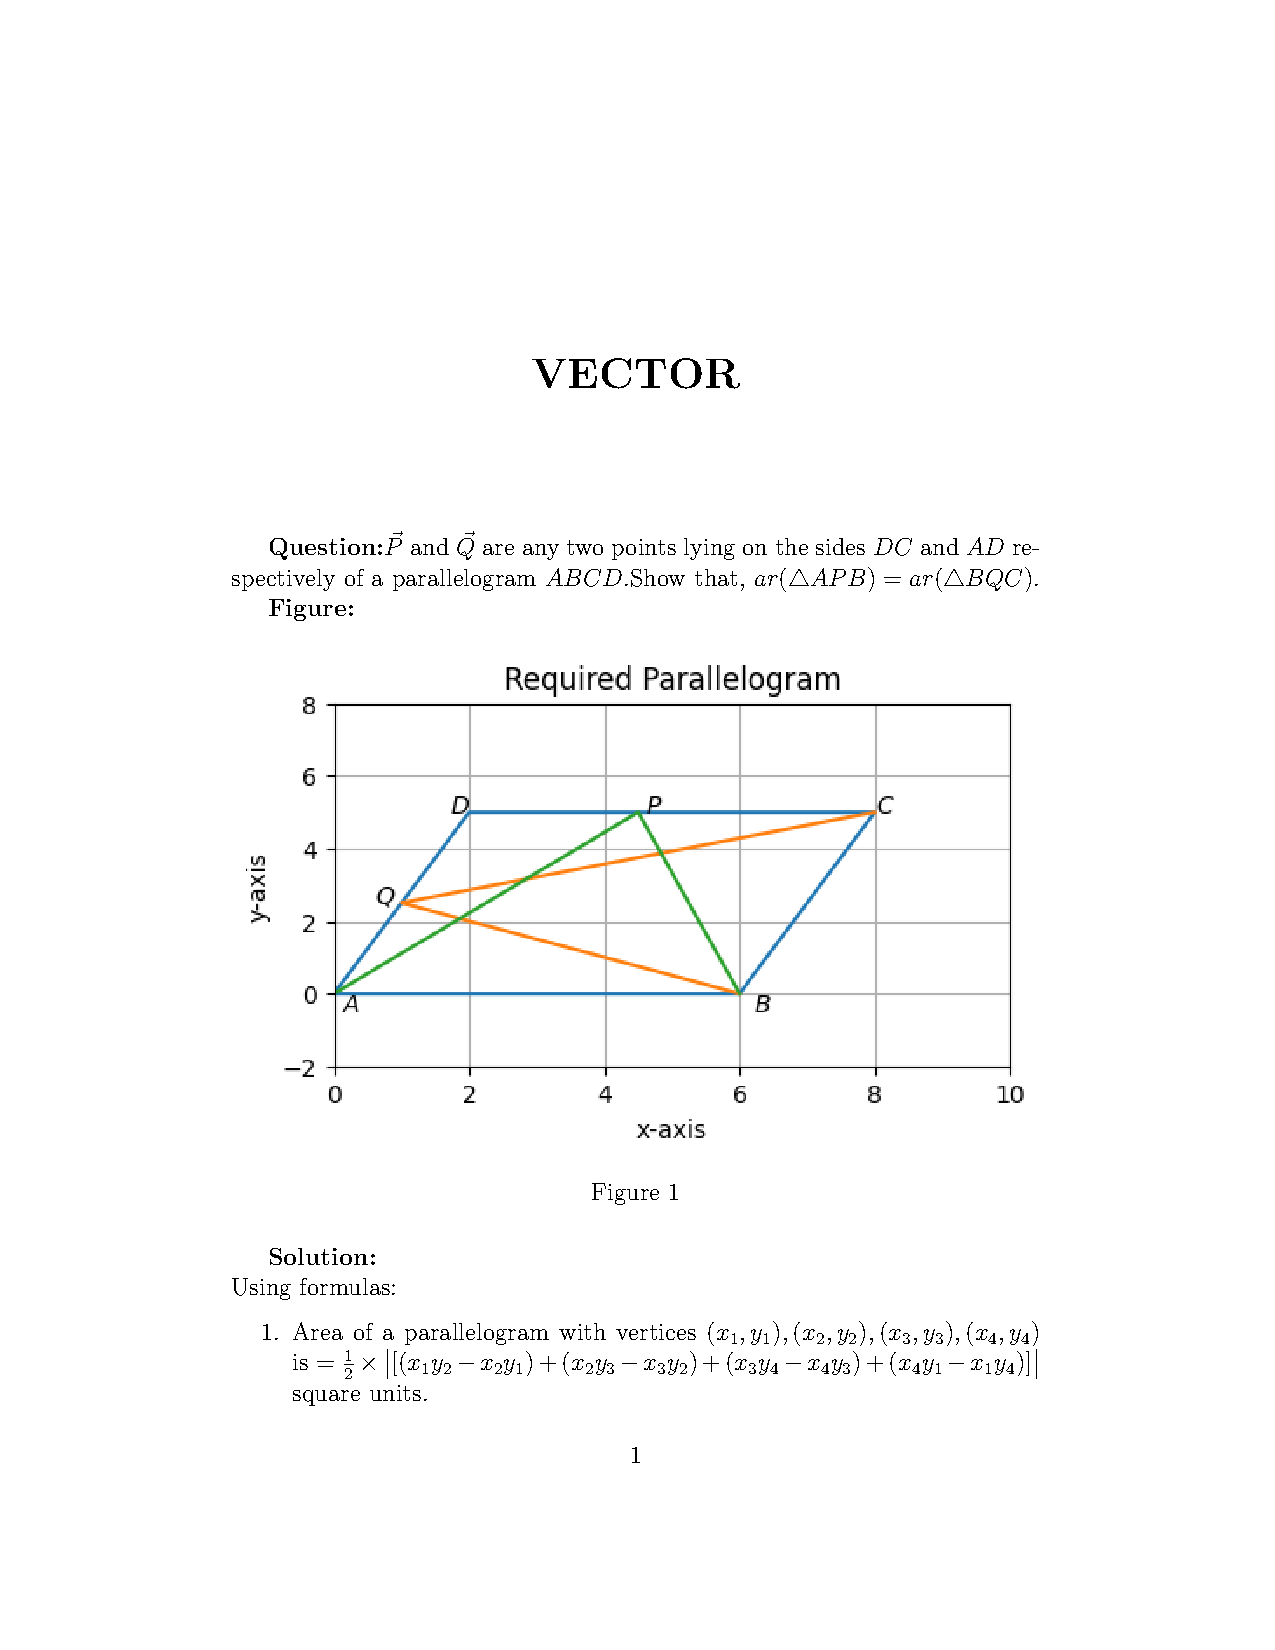
\includegraphics{fig/1.png}
    \caption{}
    \label{fig:fig:1}
\end{figure}


\textbf{Solution:}\\
Using formulas: \begin{enumerate}
\item Area of a parallelogram with  vertices $(x_1,y_1),(x_2,y_2),(x_3,y_3),(x_4,y_4)$ is =  $\frac{1}{2}\times \big |[(x_1y_2-x_2y_1)+(x_2y_3-x_3y_2)+(x_3y_4-x_4y_3)+(x_4y_1-x_1y_4)] \big|$ square units.
\item Area of a triangle with vertices $(x_1,y_1),(x_2,y_2),(x_3,y_3)$ is =  $\frac{1}{2}\times \big |x_1(y_2-y_3)+x_2(y_3-y_1)+x_3(y_1-y_2) \big|$ square units.

\item If a triangle and a parallelogram are on the same base and between the same parallels, then area of the triangle is equal to half the area of the parallelogram.

\end{enumerate}
From \figref{fig:1} ,
considering $\triangle BQC$ and parallelogram $ ABCD$, having \underline{same base $BC$} and, \underline{$AD$ is parallel to $BC$}.\\

\begin{equation}
\implies \triangle BQC = \frac{1}{2}\times ar ABCD.
 \label{eq:eq:1}
\end{equation}

Considering $\triangle APB$ and parallelogram $ABCD$ , having \underline{same base $AB$} and,\underline{$DC$ is parallel to $AB$}.

\begin{equation}
\implies \triangle APB = \frac{1}{2}\times ar ABCD.
 \label{eq:eq:2}
\end{equation}

By comparing \eqref{eq:1} and \eqref{eq:2} we obtain that,

\begin{equation}
    ar(\triangle APB) =  ar(\triangle BQC).
\end{equation}
\begin{center}
 Hence proved.

\end{center}

\textbf{Proof by the help of diagram :}(\figref{fig:1})\\
For the $\triangle APB$, the vertices of the triangle are

   $\Vec{A}=\begin{pmatrix}
       0\\0
   \end{pmatrix},
   \Vec{P}=\begin{pmatrix}
       4.5\\5
   \end{pmatrix},
   \Vec{B}=\begin{pmatrix}
       6\\0
   \end{pmatrix}$

   
$\implies \triangle APB = \frac{1}{2}\times \big |x_1(y_2-y_3)+x_2(y_3-y_1)+x_3(y_1-y_2) \big|$\\
$ = \frac{1}{2} \times \big |0(5-0)+4.5(0-0)+6(0-5)\big|\\
 = \frac{1}{2} \times\big |0+0-30\big|\\
 =\frac{1}{2} \times30\\
 =15 $ square units.


 For the $\triangle BQC$, the vertices of the triangle are
 
   $\Vec{B}=\begin{pmatrix}
       6\\0
   \end{pmatrix},
   \Vec{Q}=\begin{pmatrix}
       1\\2.5
   \end{pmatrix},
   \Vec{C}=\begin{pmatrix}
       8\\5
   \end{pmatrix}$

   
$\implies \triangle BQC = \frac{1}{2}\times \big |x_1(y_2-y_3)+x_2(y_3-y_1)+x_3(y_1-y_2) \big|$\\
$ = \frac{1}{2} \times \big |6(2.5-5)+1(5-0)+8(0-2.5)\big|\\
 = \frac{1}{2} \times\big |-15+5-20\big|\\
 =\frac{1}{2} \times30\\
 =15 $ square units.

 
  For parallelogram $ABCD$,the vertices are

   $\Vec{A}=\begin{pmatrix}
       0\\0
   \end{pmatrix},
 \Vec{B}=\begin{pmatrix}
       6\\0
   \end{pmatrix},
   \Vec{C}=\begin{pmatrix}
       8\\5
   \end{pmatrix},
   \Vec{D}=\begin{pmatrix}
       2\\5
   \end{pmatrix}$
   
$\implies ar ABCD = \frac{1}{2}\times \big |[(x_1y_2-x_2y_1)+(x_2y_3-x_3y_2)+(x_3y_4-x_4y_3)+(x_4y_1-x_1y_4)] \big|$\\
$ = \frac{1}{2} \times \big |[(0.0-6.0)+(6.5-8.0)+(8.5-2.5)+(2.0-0.5)] \big|
 = \frac{1}{2} \times\big |30+30\big|\\
 =\frac{1}{2} \times60\\
 =30 $ square units.

 Therefore,$ar ABCD = \frac{1}{2}\times ar \triangle APB = \frac{1}{2}\times ar \triangle BQC$(proved).


\end{document}



